\documentclass{article}
\usepackage[utf8]{inputenc}
\usepackage{amsmath}
\usepackage{float}
\usepackage{array}
\usepackage{hyperref}
\usepackage{listings}
\usepackage{geometry}
\usepackage{graphicx}
\usepackage[spanish]{babel}


\title{ \textbf{Proyecto Final} }
\author{Martínez Ostoa Néstor Iván \\ \#315618648 \\ Arquitectura Cliente Servidor - 2946} 
\date{Agosto 2021}

\begin{document}

\maketitle


% --------------------------------------------------------------------
% --------------------------------------------------------------------
% --------------------------------------------------------------------
\section{Objetivos}

Realizar una arquitectura cliente servidor en lenguaje C para simular un manejador de base de datos. El proyecto deberá cumplir con lo siguiente: 

\begin{itemize}
    \item El cliente debe enviar un comando al servidor
    \item El servidor debe recibir las instrucciones del cliente y realizar las operaciones correspondientes
    \item El servidor deberá responderle de vuelta al cliente
	\item El servidor deberá ejecutar sus acciones sobre archivos
\end{itemize}


% --------------------------------------------------------------------
% --------------------------------------------------------------------
% --------------------------------------------------------------------
\section{Descripción de la arquitectura}

Como se mencionó en los objetivos, la idea de esta arquitectura será simular un manejador de base de datos en donde el cliente será responsable de ejecutar secuencias de SQL y el servidor de responder a dichas secuencias y manejar los archivos correspondientes de la base de datos. A continuación se especifican las responsabilidades de cada entidad. 

\subsection{Servidor}

Los comandos que el servidor reciba se ejecutarán sobre archivos y éste deberá ser capaz de procesar de manera correcta comandos como el siguiente: \\

\verb|INSERT numcta apellido_paterno apellido_materno nombre(s)| \\ 

donde \verb|numcta| es el número de cuenta del alumno a insertar en la base de datos. El servidor deberá manejar las inserciones mediante archivos cuyo nombre será el valor de \verb|numcta|. Se tendrá que tener un archivo por alumno. Una vez que se realicé la inserción, el servidor deberá responder al cliente con un mensaje de éxito o error en caso de existir uno. 


\begin{figure}[H]
    \centering
    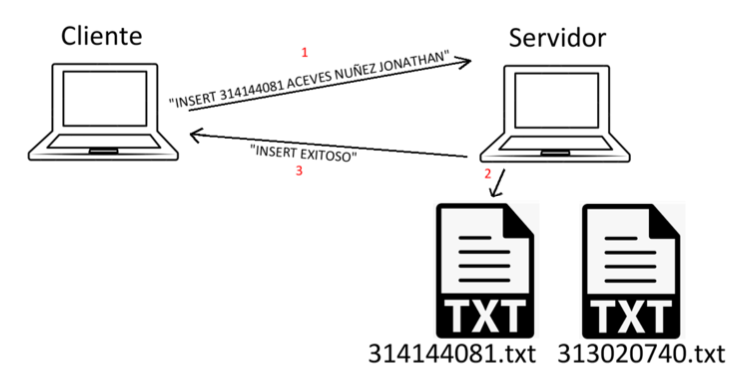
\includegraphics[scale=0.3]{imgs/insert_numcta.png}
    \caption{Ejemplo de inserción de elementos en la base de datos}
    \label{fig:insert_numcta}
\end{figure}

\subsection{Cliente}

Por otro lado, el cliente a parte de poder insertar elementos a la base de datos, será capaz de hacer selecciones con base en un número de cuenta. El cliente, por medio del comando \verb|select numcta| podrá obtener el contenido del archivo \verb|numcta|. Cuando el servidor reciba esta instrucción, deberá responder con el contenido del archivo en caso de que exista. De lo contrario, deberá mandar un mensaje de error. 

\begin{figure}[H]
    \centering
    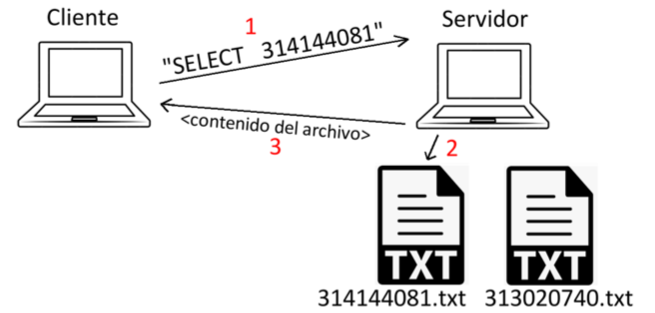
\includegraphics[scale=0.32]{imgs/select_numcta.png}
    \caption{Ejemplo de selección de elementos dentro la base de datos}
    \label{fig:select_numcta}
\end{figure}


% --------------------------------------------------------------------
% --------------------------------------------------------------------
% --------------------------------------------------------------------
\section{Desarrollo}

A continuación se muestra capturas de pantalla con las salidas de ejecución desde la terminal mostrando el funcionamiento del programa:

\begin{enumerate}
    \item Compilamos y ejecutamos el servidor
    	\begin{figure}[H]
		    \centering
		    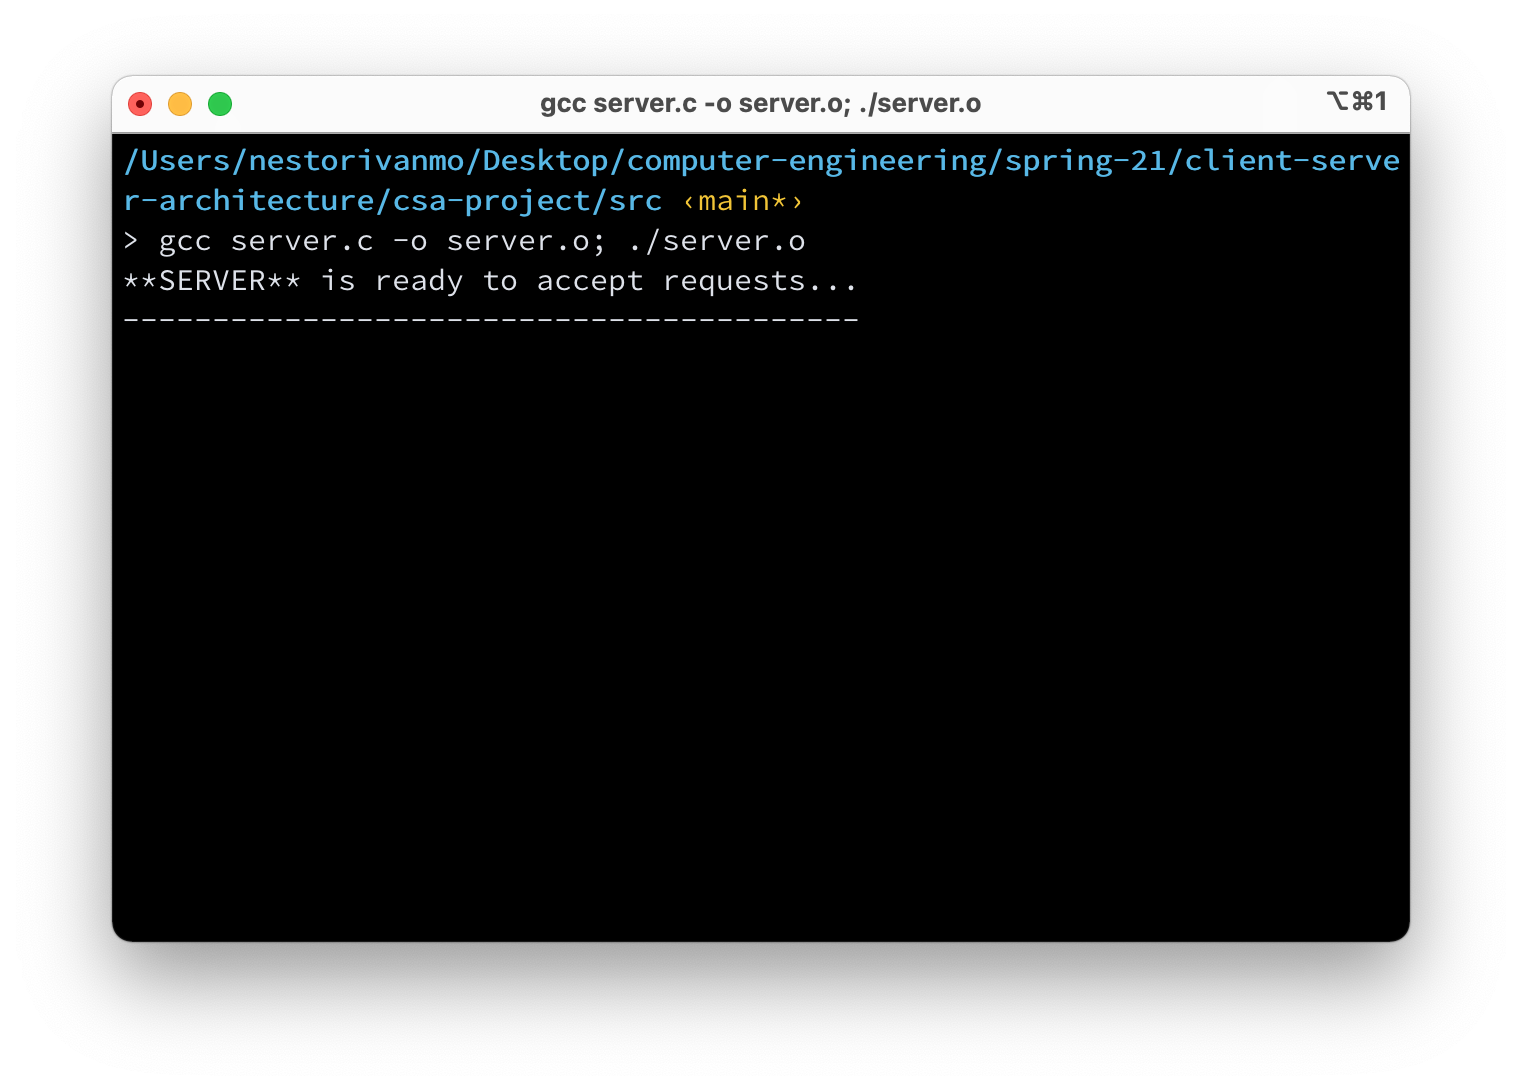
\includegraphics[scale=0.4]{imgs/server.png}
		\end{figure}
    \item Compilamos y ejecutamos el cliente con la dirección IP del host el cual queda a la espera de los comandos:
    	\begin{figure}[H]
		    \centering
		    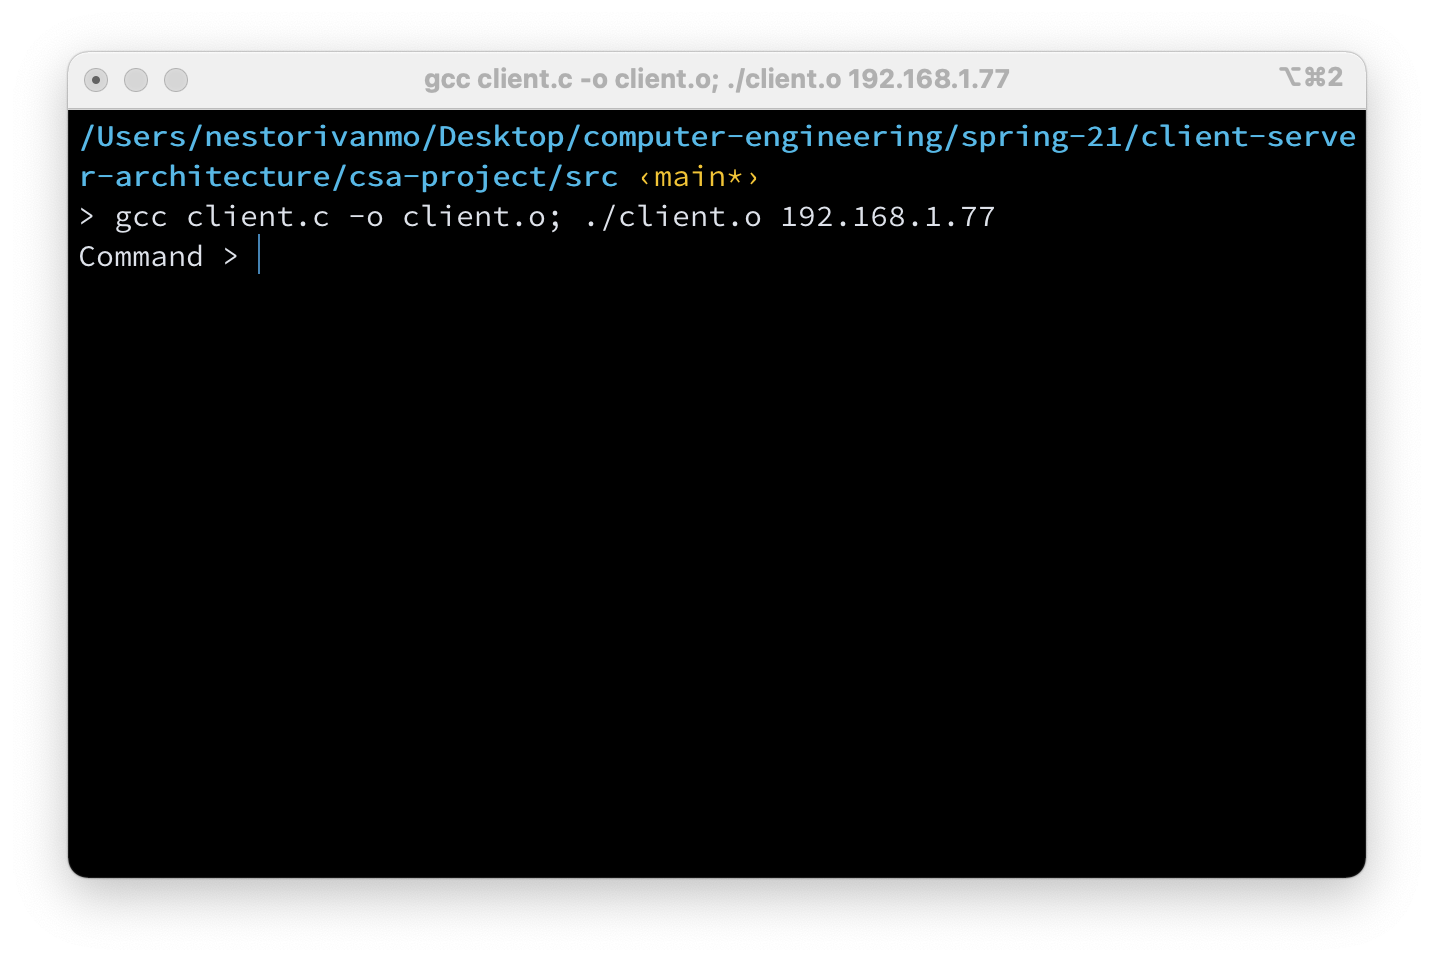
\includegraphics[scale=0.4]{imgs/client_initial.png}
		\end{figure}
	\item Inserción de un alumno
		\begin{figure}[H]
		    \centering
		    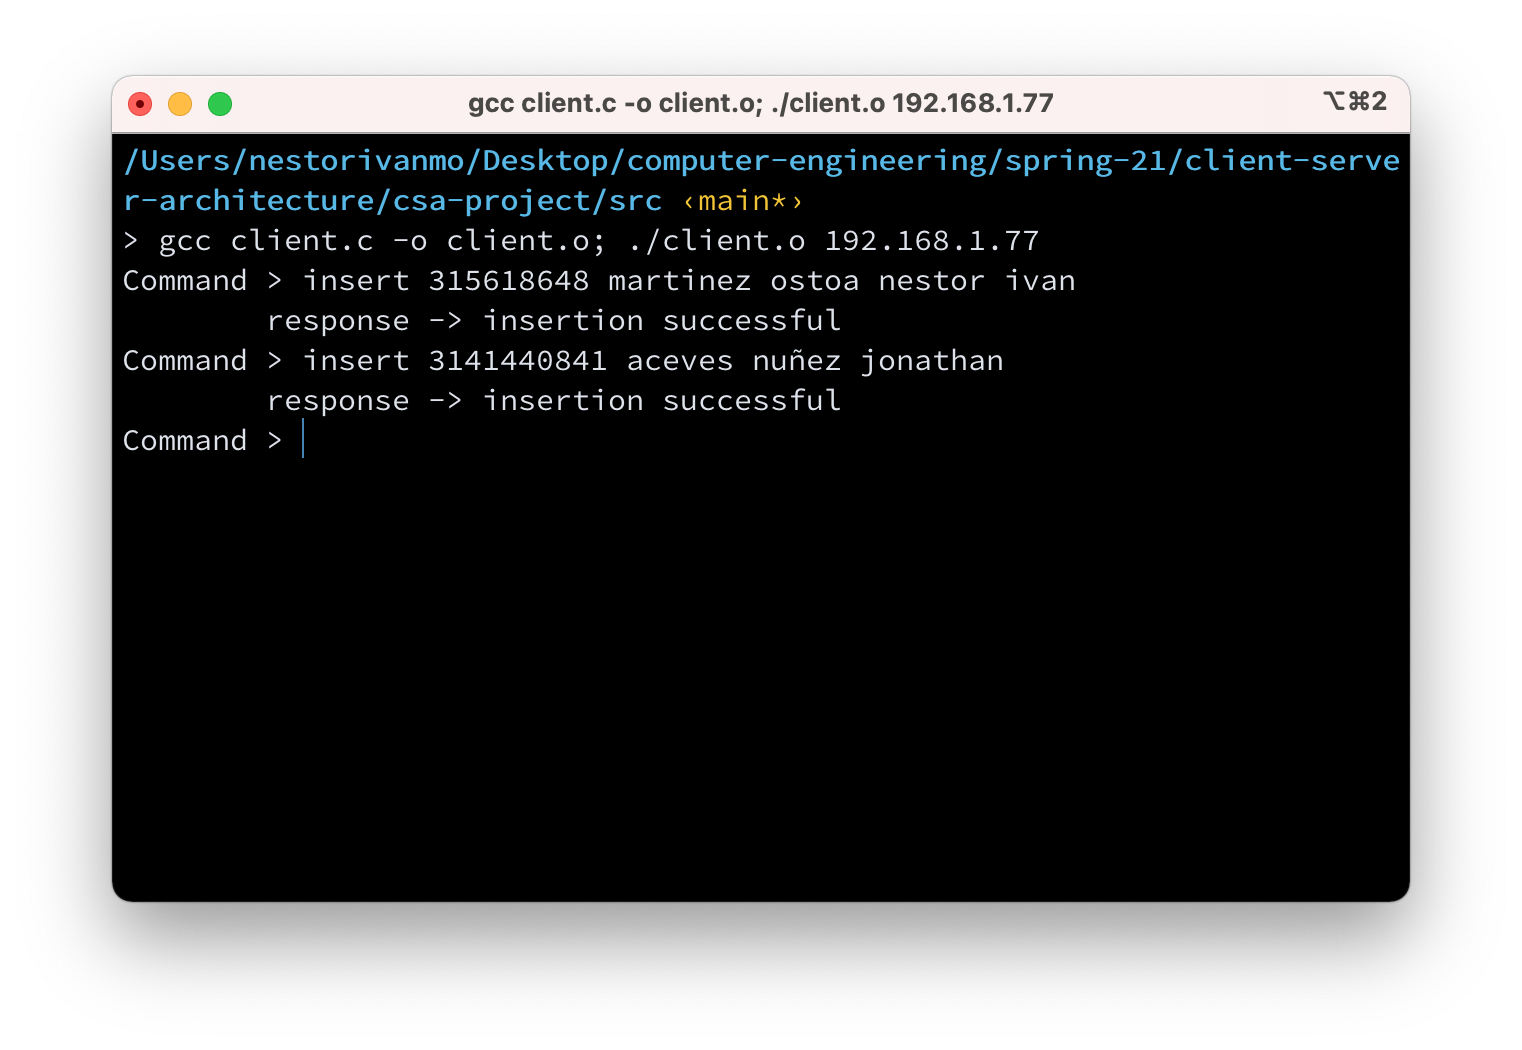
\includegraphics[scale=0.4]{imgs/client_insertion.png}
		    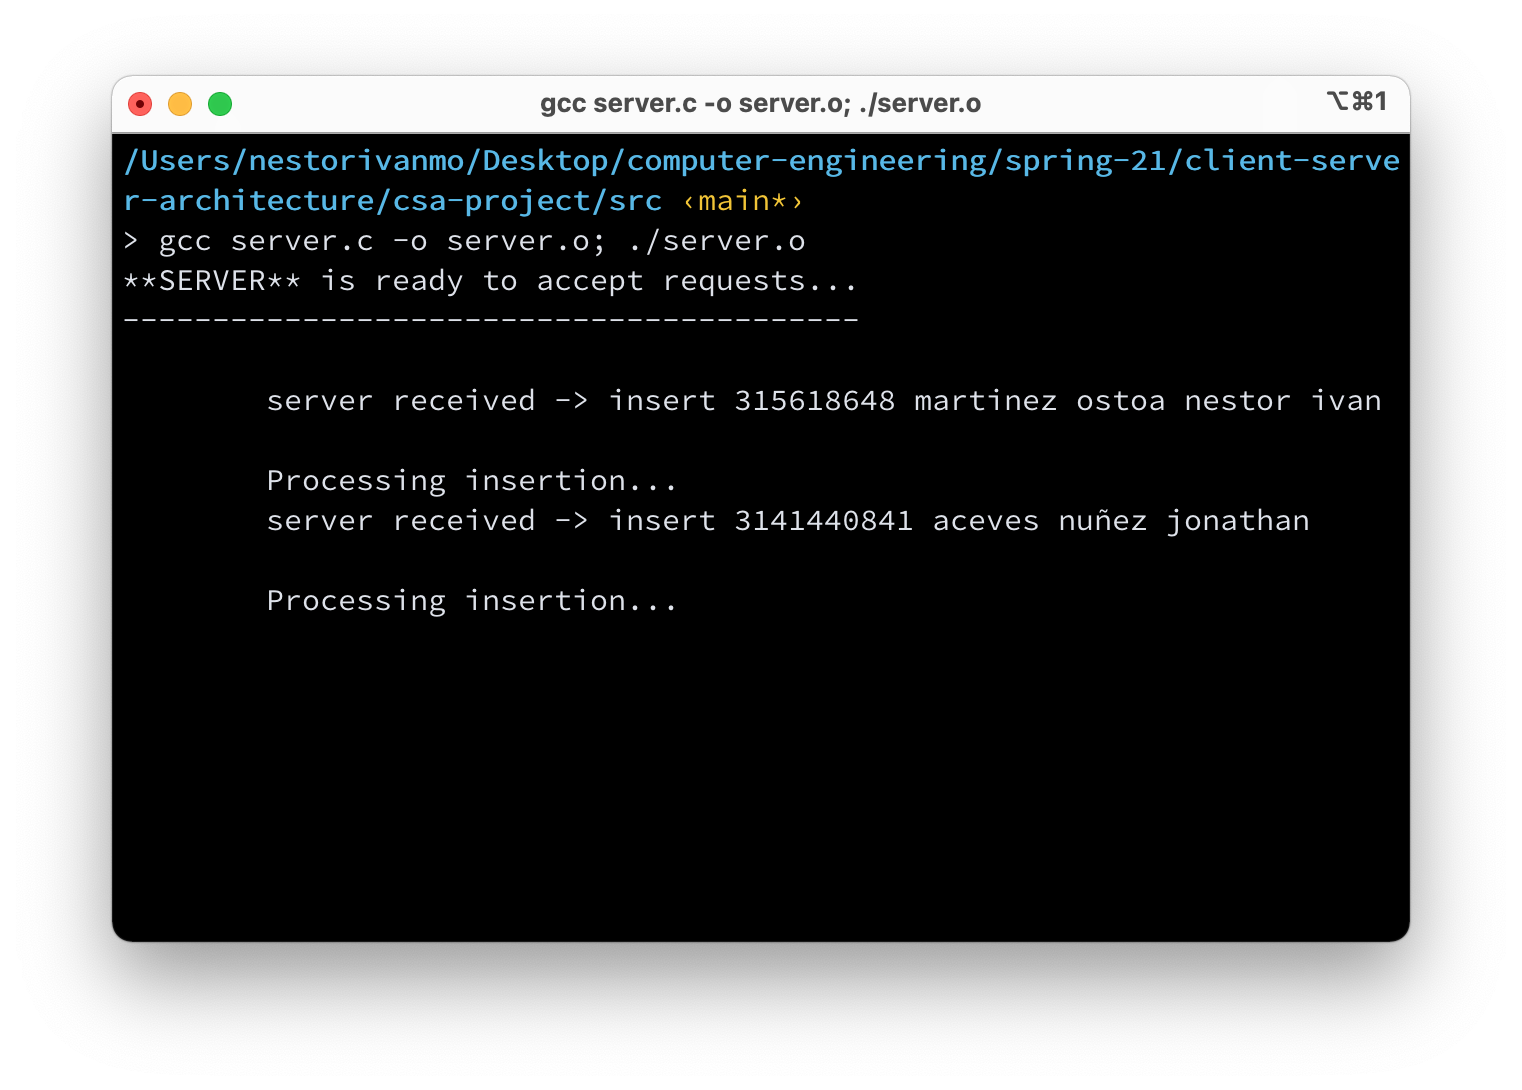
\includegraphics[scale=0.4]{imgs/server_insertion.png}		    
		\end{figure}
	\item Recuperación de los datos de un alumno
		\begin{figure}[H]
		    \centering
		    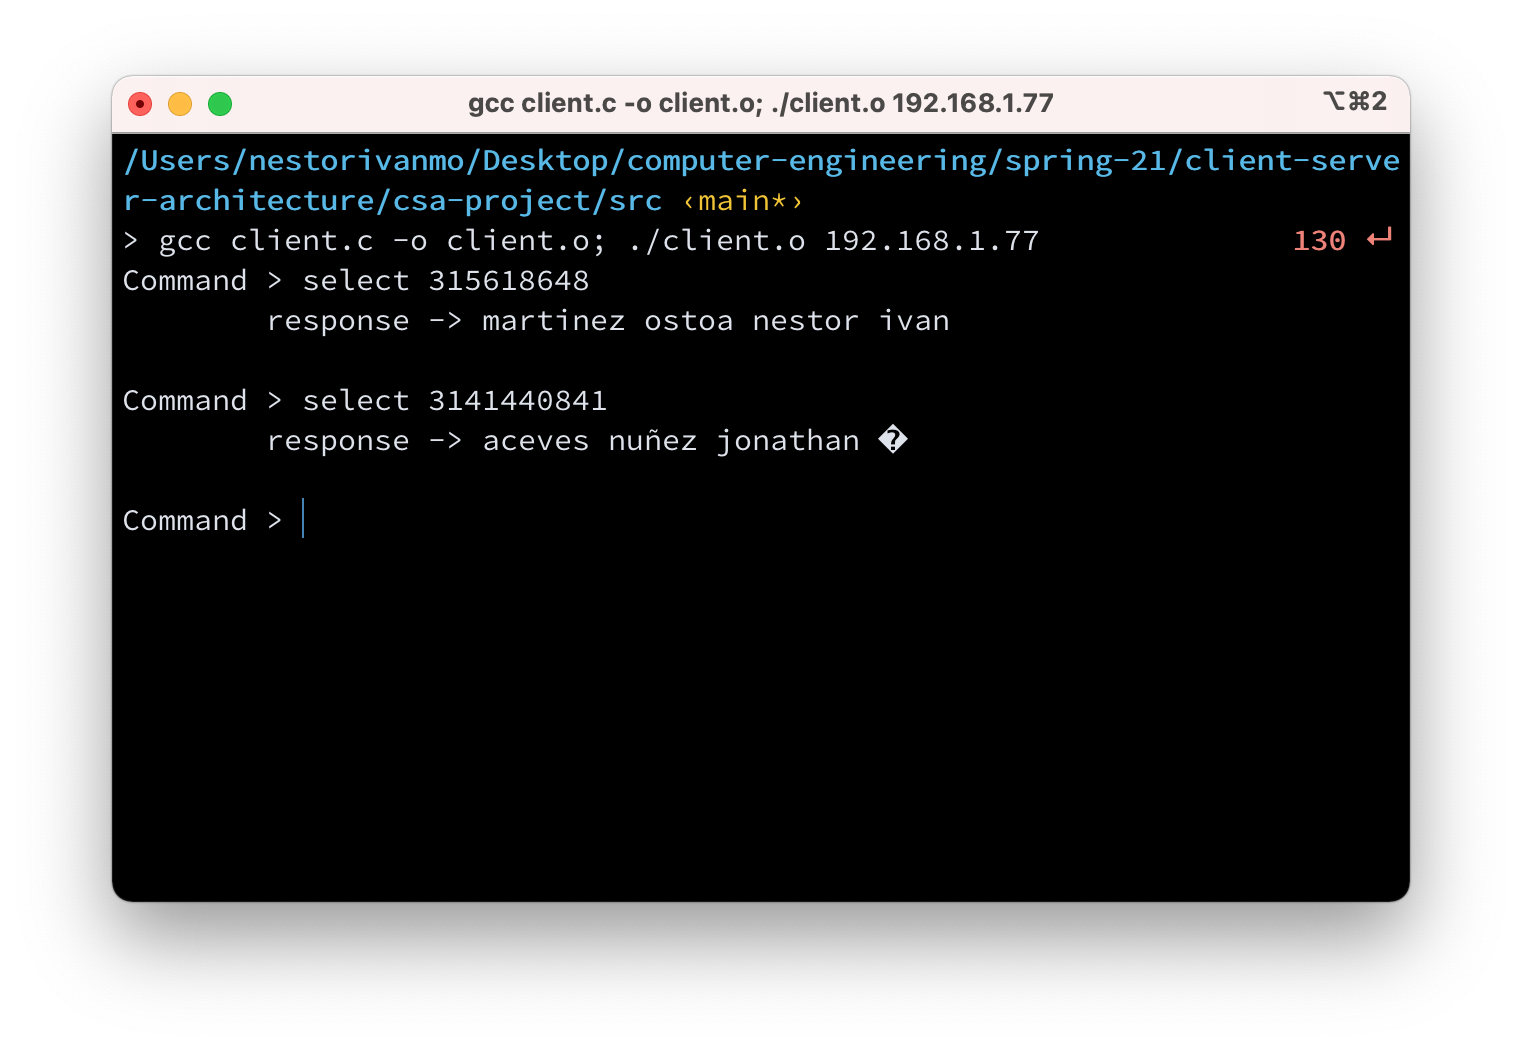
\includegraphics[scale=0.4]{imgs/client_selection.png}
		    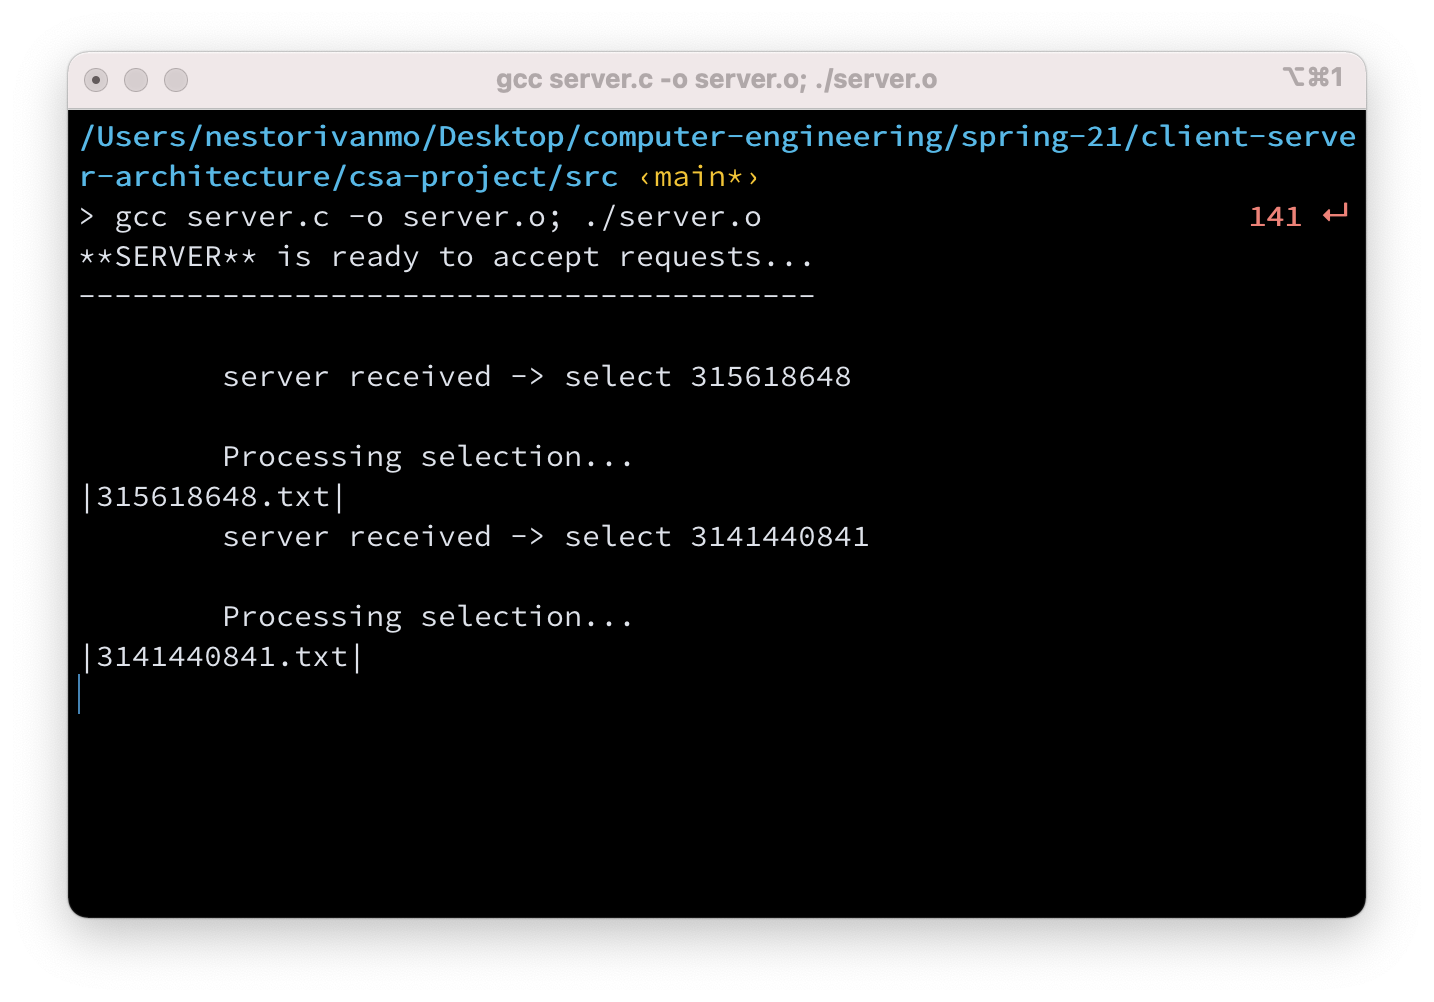
\includegraphics[scale=0.4]{imgs/server_selection}		    
		\end{figure}	
\end{enumerate}


% --------------------------------------------------------------------
% --------------------------------------------------------------------
% --------------------------------------------------------------------
\section{Código}

El código que se menciona a continuación también se puede encontrar en la siguiente \href{https://github.com/nestorivanmo/computer-engineering/tree/main/spring-21/client-server-architecture/csa-project/src}{URL}

\subsection{Servidor}
\begin{lstlisting}[language=c]
#include <stdio.h>
#include <stdlib.h>
#include <unistd.h>
#include <errno.h>
#include <string.h>
#include <ctype.h>
#include <sys/types.h>
#include <sys/socket.h>
#include <netinet/in.h>
#include <arpa/inet.h>
#include <sys/wait.h>
#include <signal.h>
#include <dirent.h>

#define PORT 3490
#define BACKLOG 10
#define MAXDATASIZE 100
#define ENTITY "**SERVER**"
#define DB_FILES_PATH "db_files"

void handle_system_call(int result, char *system_call_msg, int verbose) {
    if (result == -1) {
        perror("error: ");
        printf("%s: error at %s\n", ENTITY, system_call_msg);
        exit(1);
    }
    if (verbose == 1) {
        printf("%s: success at %s\n", ENTITY, system_call_msg);
    }
}

char *process_insertion(char instructions[][MAXDATASIZE]) {
    char *account_number = instructions[1];
    char *first_last_name = instructions[2];
    char *second_last_name = instructions[3];
    char *first_name = instructions[4];
    char *middle_name = instructions[5];
    
    FILE *fp;
    char file[100];
    sprintf(file, "%s.txt", account_number);
    fp = fopen(file, "w");

    if (fp == NULL) {
        return "insertion failed...";
    }

    fflush(stdin);
    fprintf(fp, "%s %s %s %s", first_last_name, second_last_name, first_name, middle_name);
    fclose(fp);

    return "insertion successful";
}

char* process_selection(char account_number[MAXDATASIZE]) {
    char num_cta[MAXDATASIZE];
    
    int j = 0;
    for (j = 0; j < MAXDATASIZE; j++)
        num_cta[j] = '\0';

    int i = 0;
    int digit_idx = 0;
    for (i = 0; i < MAXDATASIZE; i++) {
        if (isdigit(account_number[i])) {
            num_cta[digit_idx] = account_number[i];
            digit_idx++;
        }
    }
    
    int idx = 0;
    char extension[4] = ".txt";
    for (i = digit_idx; i < digit_idx + 4; i++) {
        num_cta[i] = extension[idx];
        idx++;
    }

    printf("|%s|\n", num_cta);
        
    FILE *fp;
    fp = fopen(num_cta, "r");
    if (fp == NULL) {
        return "error reading file";
    }

    char fln[MAXDATASIZE];
    char sln[MAXDATASIZE];
    char fn[MAXDATASIZE];
    char mn[MAXDATASIZE];
    fscanf(fp, "%s %s %s %s", fln, sln, fn, mn);

    static char db_result[MAXDATASIZE];
    sprintf(db_result, "%s %s %s %s\n", fln, sln, fn, mn);

    //printf("%s\n", db_result);

    return db_result;
}

char *process_request(char *buffer) {
    printf("\tserver received -> %s\n", buffer);

    char instructions[10][MAXDATASIZE];
    int idx = 0;

    char *pch = strtok(buffer, " ");
    while (pch != NULL) {
        strcpy(instructions[idx], pch);
        pch = strtok(NULL, " ");
        idx++;
    }
    
    if (strcmp(instructions[0], "insert") == 0) {
        printf("\tProcessing insertion...\n");
        return process_insertion(instructions);
    } else if (strcmp(instructions[0], "select") == 0) {
        printf("\tProcessing selection...\n");
        return process_selection(instructions[1]);
    } else if (strcmp(instructions[0], "exit") == 10) {
        return "bye";
    } else  {
        return strcat(instructions[0], " not recognized");
    }
}

void accept_requests(int server_socket_fd, int verbose) {
    char buffer[MAXDATASIZE];
    int bytes_received;
    char *response;
    
    //ACCEPT()
    int client_socket_fd;
    struct sockaddr_in client_ip_addr;
    unsigned int sockaddr_in_size = sizeof(client_ip_addr);
    client_socket_fd = accept(
        server_socket_fd, (struct sockaddr*)&client_ip_addr, &sockaddr_in_size
    );
    handle_system_call(client_socket_fd, "ACCEPT()", verbose);

    while (1) {

        //RECV()
        if((bytes_received = recv(client_socket_fd, buffer, MAXDATASIZE-1, 0)) == -1){ 
            perror("SERVER recv()");
        } else {
            buffer[bytes_received] = '\0';
            if (strlen(buffer) > 1) {
                response = process_request(buffer);
            }
        }

        //SEND()
        if (send(client_socket_fd, response, strlen(response), 0) == -1) {
            printf("%s: SEND() error\n", ENTITY);
        }
    }  
}

int main(int argc, char *argv[ ]){
    int verbose = 0;
    int system_call_result;

    printf("%s is ready to accept requests...\n-----------------------------------------\n\n", ENTITY);

    //SOCKET()
    int server_socket_fd;
    int domain = PF_INET;
    int type = SOCK_STREAM;
    int protocol = 0;
    server_socket_fd = socket(domain, type, protocol);
    handle_system_call(server_socket_fd, "SOCKET()", verbose);

    //BIND()
    int yes=1;
    if (setsockopt(server_socket_fd, SOL_SOCKET,SO_REUSEADDR, &yes, sizeof yes) == -1) {
        perror("setsockopt");
        exit(1);
    }
    struct sockaddr_in server_ip_addr;
    server_ip_addr.sin_family = AF_INET;
    server_ip_addr.sin_port = htons(PORT);
    server_ip_addr.sin_addr.s_addr = INADDR_ANY;
    memset(&(server_ip_addr.sin_zero), '\0', 8);
    system_call_result = bind(
        server_socket_fd, (struct sockaddr*)&server_ip_addr, 
        sizeof(struct sockaddr)
    );
    handle_system_call(system_call_result, "BIND()", verbose);

    //LISTEN()
    system_call_result = listen(server_socket_fd, BACKLOG);
    handle_system_call(system_call_result, "LISTEN()", verbose);

    //CLIENT SERVER INTERACTION
    accept_requests(server_socket_fd, verbose);

    //CLOSE()
    close(server_socket_fd);

    return 0;
}\end{lstlisting}


\subsection{Cliente}

\begin{lstlisting}[language=c]
#include <stdio.h>
#include <stdlib.h>
#include <unistd.h>
#include <errno.h>
#include <string.h>
#include <netdb.h>
#include <sys/types.h>
#include <netinet/in.h>
#include <sys/socket.h>

#define PORT 3490
#define MAXDATASIZE 1024
#define ENTITY "**CLIENT**"

void handle_system_call(int result, char *system_call_msg, int verbose) {
    if (result == -1) {
        printf("%s: error at %s\n", ENTITY, system_call_msg);
        exit(1);
    }
    if (verbose == 1) {
        printf("%s: success at %s\n", ENTITY, system_call_msg);
    }
}

void handle_client_input_parameters(int argc, char *ip_address, int verbose) {
    if (ip_address == NULL) {
        printf("%s: missing ip address\n", ENTITY);
        exit(1);
    }
    if (verbose == 1){
        printf("%s: input parameters are ok!\n", ENTITY);
    }
}

void verify_host_name(struct hostent *he, int verbose) {
    if (he == NULL) {
        printf("%s: error at GETHOSTBYNAME()\n", ENTITY);
        exit(1);
    }
    if (verbose == 1){
        printf("%s: success at GETHOSTBYBNAME()\n", ENTITY);
    }
}

char *read_string(char *msg) {
    char *str;
    char buf[MAXDATASIZE]; 
    printf("%s", msg);
    fgets(buf, MAXDATASIZE, stdin);
    str = (char*) malloc(strlen(buf) + 1);
    if (str == NULL) {
       printf("%s: error out of memory\n", ENTITY);
       exit(1);
    }
    strcpy(str, buf);
    return str;
}

char *handle_server_msgs(char *buffer) {
    printf("\tresponse -> %s\n", buffer);
    return "";
}

void handle_connection_with_server(int client_socket_fd, int verbose) {
    char buffer[MAXDATASIZE];
    int bytes_received;

    char stop_command[] = "exit";
    char command[MAXDATASIZE];
    do {
        printf("Command > ");
        fflush(stdout);
        fgets(command, MAXDATASIZE, stdin);

        //SEND()
        if(send(client_socket_fd, command, strlen(command), 0) == -1) {
            printf("%s: SEND() error\n", ENTITY);
        }

        //RECV()
        if((bytes_received = recv(client_socket_fd, buffer, MAXDATASIZE-1, 0)) == -1){
            printf("%s: RECV() error\n", ENTITY);
        }
        buffer[bytes_received] = '\0';
        char *response = handle_server_msgs(buffer);

    } while (strcmp(command, stop_command) != 10);

}

int main(int argc, char *argv[]){
    int verbose = 0;
    int system_call_result;

    //VERIFY CORRECT INPUT PARAMETERS    
    char *client_input_ip_addr = argv[1];
    handle_client_input_parameters(argc, client_input_ip_addr, verbose);

    //HOSTBYNAME
    struct hostent *he;
    he = gethostbyname(client_input_ip_addr);
    verify_host_name(he, verbose);

    //SOCKET()
    int client_socket_fd;
    int domain = PF_INET;
    int type = SOCK_STREAM;
    int protocol = 0;
    client_socket_fd = socket(domain, type, protocol);
    handle_system_call(client_socket_fd, "SOCKET()", verbose);

    //CONNECT()
    struct sockaddr_in server_ip_addr;
    server_ip_addr.sin_family = AF_INET;
    server_ip_addr.sin_port = htons(PORT);
    server_ip_addr.sin_addr = *((struct in_addr *)he->h_addr);
    memset(&(server_ip_addr.sin_zero), '\0', 8);
    system_call_result = connect(
        client_socket_fd, (struct sockaddr*)&server_ip_addr,
        sizeof(struct sockaddr)
    );
    handle_system_call(system_call_result, "CONNECT()", verbose);

    //connect with server
    handle_connection_with_server(client_socket_fd, verbose);

    //CLOSE()
    close(client_socket_fd);

    return 0;
}\end{lstlisting}



% --------------------------------------------------------------------
% --------------------------------------------------------------------
% --------------------------------------------------------------------
\section{Conclusiones}

Con el desarrollo de este proyecto se pudieron cumplir de manera eficiente los objetivos planteados: programar una arquitectura cliente servidor utilizando sockets. Si bien lo más difícil de este proyecto, en teoría, era la programación de los sockets, lo que más tiempo me tomó resolver fue la lectura y escritura de archivos pues el manejo de cadenas de texto en C no es muy transparente. Independientemente de esto, el proyecto fungió como una parte importante en el entendimiento de las arquitecturas cliente-servidor así como la programación de sockets en UNIX.


% --------------------------------------------------------------------
% --------------------------------------------------------------------
% --------------------------------------------------------------------
\begin{thebibliography}{}

\bibitem{zamitiz} Zamitiz C. (2021). Apuntes de la materia Arquitectura Cliente Servidor. Facultad de Ingeniería. UNAM

\bibitem{zamitiz} Hall, B. (2019). Beej’s Guide to Network Programming. Independently Published.

\end{thebibliography} 


\end{document}










